% !TEX program = xelatex

\documentclass[10pt,a4paper]{article}
\usepackage[top = 1.5cm, bottom = 1.5cm, left = 1.5cm, right = 1.5cm]{geometry}

\usepackage{titling}
\usepackage[czech]{babel}
\usepackage{graphicx}
\usepackage{lmodern}
\usepackage{hyperref}
\usepackage{setspace}
\usepackage{csvsimple}

\usepackage{amsmath}
\usepackage{amssymb}
\usepackage{gensymb}
\usepackage{mathtools}
\usepackage{units}
\usepackage{bm}
\delimitershortfall=-1pt

\usepackage{gnuplottex}
\usepackage{epstopdf}

% no page break
\newenvironment{absolutelynopagebreak}
  {\par\nobreak\vfil\penalty0\vfilneg
   \vtop\bgroup}
  {\par\xdef\tpd{\the\prevdepth}\egroup
   \prevdepth=\tpd}


% redefine \sqrt
\usepackage{letltxmacro}
\makeatletter
\let\oldr@@t\r@@t
\def\r@@t#1#2{%
\setbox0=\hbox{$\oldr@@t#1{#2\,}$}\dimen0=\ht0
\advance\dimen0-0.2\ht0
\setbox2=\hbox{\vrule height\ht0 depth -\dimen0}%
{\box0\lower0.4pt\box2}}
\LetLtxMacro{\oldsqrt}{\sqrt}
\renewcommand*{\sqrt}[2][\ ]{\oldsqrt[#1]{#2\,}\,}
\makeatother

\DeclarePairedDelimiter\ceil{\lceil}{\rceil}
\DeclarePairedDelimiter\floor{\lfloor}{\rfloor}

\LetLtxMacro{\oldhbar}{\hbar}
\AtBeginDocument{\renewcommand*{\hbar}{{\mkern-1mu\raisebox{-0.055em}{$\mathchar'26$}\mkern-8mu\mathrm{h}}}}

\def\ph{\phantom}
\def\vph{\vphantom}
\def\hph{\hphantom}
\def\rzw{\mathrlap}
\def\lzw{\mathllap}
\def\czw{\mathclap}

\def\?{\mathit{?}}

\def\+{+\!\!}
\def\-{-\!\!}

\newcommand{\comm}[2]{\left[ #1, #2 \right]}
\newcommand{\const}[1]{\text{#1}}
\newcommand{\norm}[1]{\left\lVert#1\right\rVert}

\newcommand{\mat}[1]{
    \begin{pmatrix}
        #1
    \end{pmatrix}
}

\newcommand{\mata}[2]{
    \left(
    \begin{array}{@{}#1@{}}
        #2
    \end{array}
    \right)
}

\newcommand{\smat}[2][1]{
    \scalebox{#1}{$\mat{#2}$}
}

\renewcommand{\d}[1]{\;\const{d}#1}
\newcommand{\dd}[2]{\frac{\const{d} #1}{\const{d} #2} \;}
\newcommand{\pd}[2]{\frac{\partial  #1}{\partial  #2} \;}

\newcommand{\bra}[1]{\left< #1 \right|}
\newcommand{\ket}[1]{\left| #1 \right>}
\newcommand{\braket}[2]{\left< #1 \middle| #2 \right>}

\newcommand{\bhat}[1]{\hat{\bm{#1}}}

\newcommand{\e}[1]{\const{e}^{#1}}
\renewcommand{\i}{\const{i}}

\begin{document}

\title{Kvantová mechanika I: Domácí úkoly}
\author{Michal Grňo}
\date{\today}

\maketitle

\section{Cvičení 13. 11.}

\subsection{Zadání}
Vodík se skládá z protonu (spin ½) a elektronu (spin ½) v orbitalu \textit{d} (tedy $\ell=2$). Operátor celkového momentu hybnosti je
\begin{gather*}
    \bhat{J} = \bhat{S}^{(\const{p})} + \bhat{S}^{(\const{e})} + \bhat{L}
\end{gather*}
Kolika různých kvantových stavů může systém nabývat? Jakých hodnot může nabývat celkový moment hybnosti $j$ a kolik stavů každé z nich přísluší?

Určete normalizované stavy $\ket{j \; m} \in \left\{ \ket{3 \; 3}, \ket{3 \; 2}, \ket{3 \; 1} \right\}$. Určete střední hodnotu $\bra{3 \; 2} \bhat{S}^{(\const{e})} \cdot \bhat{S}^{(\const{p})} \ket{3 \; 2}$.

\subsection{Řešení}
Protože se jedná o rozlišitelné veličiny (spin protonu dokážeme odlišit od spinu elektronu, spin dokážeme odlišit od orbitální hybnosti), prostor kvantových stavů bude tenzorovým součinem stavů jednotlivých podsystémů. Jeho bázi tvoří kety
\begin{gather*}
    \ket{m_\const{p} \; m_e \; m_\ell} = \ket{s_\const{p} \; m_\const{p}} \otimes \ket{s_\const{e} \; m_\const{e}} \otimes \ket{\ell \; m_\ell}.
\end{gather*}
Protože $s_\const{p} = s_\const{e} = \nicefrac{1}{2}$, kvantová čísla $m_\const{p}$ a $m_\const{e}$ mohou nabývat pouze hodnoty $\pm \nicefrac{1}{2}$. Kvantové číslo $m_\ell \in \left\{ -2, -1, 0, 1, 2 \right\}$. Celkem má tedy systém $2 \times 2 \times 5 = 20$ stavů.

Nejprve sečteme dohromady spiny protonu a elektronu: $\bhat{S} = \bhat{S}^{(\const{p})} + \bhat{S}^{(\const{e})}$. Celkový spin musí být $\left| \frac{1}{2} - \frac{1}{2} \right| \leq s \leq \frac{1}{2} + \frac{1}{2}$, může tedy nabývat hodnoty $s=0$ nebo $s=1$. Pro jeho projekci do osy z platí $-s \leq m_\const{s} \leq s$, máme tedy celkem čtyři stavy:
\begin{gather*}
    \ket{s \; m_\const{s}} \in \left\{
        \ket{0 \; \ph{\+} 0}, \;
        \ket{1 \; \- 1}, \;
        \ket{1 \; \ph{\+} 0}, \;
        \ket{1 \; \+ 1}
    \right\}.
\end{gather*}
Dále sečteme spin s orbitalovou hybností: $\bhat{J} = \bhat{S} + \bhat{L}$. Pro celkový moment hybnosti odpovídající spinu $s=0$ platí $j=2$, $m \in \{-2, -1, 0, 1, 2\}$. Pro moment hybnosti odpovídající spinu $s=1$ platí $j \in \{1, 2, 3\}$, $m \in \{-j, ..., j\}$. Spočítáme-li, kolik stavů odpovídá jednotlivým $j$, dostaneme:
\begin{table}[!ht]
    \centering
    \begin{tabular}{ r|l }
        $\bm{j}$ &
        \bfseries počet stavů \\\hline
        1 & 3 \\
        2 & $5 + 5 = 10$ \\
        3 & 7
    \end{tabular}
\end{table}
\\
Tyto stavy budeme značit $\ket{j \; m}$, ačkoliv je pro $j=2$ toto značení ambivalentní (může označovat stav $s=0$, nebo $s=1$). Pokračujeme určením Clebsch-Gordanových koeficientů. Víme, že nejvyšší stav může být vytvořen pouze takto:
\begin{align*}
    \ket{j \; m} &= \ket{m_\const{p} \; m_\const{e} \; m_\ell} \\
    \ket{ \rzw{3}\ph{j} \; \rzw{3}\ph{m} } &= \ket{ \rzw{\nicefrac{1}{2}} \ph{m_p} \; \rzw{\nicefrac{1}{2}} \ph{m_e} \; \rzw{2} \ph{m_\ell} }
    = \ket{\uparrow \; \uparrow 2}
\end{align*}
Snadno se ověří, že $\hat{J}_{-} = \hat{S}_{-}^{(\const{p})} + \hat{S}_{-}^{(\const{e})} + \hat{L}_{-}$. Tuto rovnici můžeme použít k vyjádření dalších stavů (ve výpočtu ignorujeme faktor $\hbar$, který se nakonec zkrátí):
\begin{align*}
    \hat{J}_{-} \ket{3 \; 3} &= \left( \hat{S}_{-}^{(\const{p})} + \hat{S}_{-}^{(\const{e})} + \hat{L}_{-} \right) \ket{ \uparrow \; \uparrow 2}\\
    \sqrt{3 (3+1) - 3 (3-1)} \ket{3 \; 2} &= \ket{\downarrow \; \uparrow 2} + \ket{\uparrow \; \downarrow 2} + \sqrt{6 - 2(2-1)} \ket{\uparrow \; \uparrow 1} \\
    \oldsqrt{6} \; \ket{3 \; 2} &= \ket{\downarrow \; \uparrow 2} + \ket{\uparrow \; \downarrow 2} + 2 \ket{\uparrow \; \uparrow 1} \\[5pt]
    \ket{ 3 \; 2 } &= \frac{1}{\oldsqrt{6}} \left( \ket{\downarrow \; \uparrow 2} + \ket{\uparrow \; \downarrow 2} + 2 \ket{\uparrow \; \uparrow 1} \right).
\end{align*}
Pokračujeme vypočtením $\ket{3 \; 1}$:
\begin{align*}
    \hat{J}_{-} \ket{3 \; 2} &= \left( \hat{S}_{-}^{(\const{p})} + \hat{S}_{-}^{(\const{e})} + \hat{L}_{-} \right) \; \frac{1}{\oldsqrt{6}} \left( \ket{\downarrow \; \uparrow 2} + \ket{\uparrow \; \downarrow 2} + 2 \ket{\uparrow \; \uparrow 1} \right)
    \\
    \oldsqrt{6} \; \sqrt{3(3+1) - 2(2-1)} \; \ket{3 \; 1} &= \left( \hat{S}_{-}^{(\const{p})} + \hat{S}_{-}^{(\const{e})} + \hat{L}_{-} \right) \; \left( \ket{\downarrow \; \uparrow 2} + \ket{\uparrow \; \downarrow 2} + 2 \ket{\uparrow \; \uparrow 1} \right)
    \\[5pt]
    2 \oldsqrt{15} \; \ket{3 \; 1} &=
    0 \, \ket{\downarrow \; \uparrow 2} +
    \ph{0} \, \ket{\downarrow \; \downarrow 2} +
    2 \, \ket{\downarrow \; \uparrow 1} + \\
    &+ \ph{0} \; \ket{\downarrow \; \downarrow 2} +
    0 \, \ket{\uparrow \; \downarrow 2} +
    2 \, \ket{\uparrow \; \downarrow 1} + \\
    &+ 2 \, \ket{\downarrow \; \uparrow 1} +
    2 \, \ket{\uparrow \; \downarrow 1} +
    \sqrt{6 - 1(1-1)} \, \ket{\uparrow \; \uparrow 0}
    \\[5pt]
    \ket{3 \; 1} &= \frac{1}{\oldsqrt{15}} \left(
        \ket{\downarrow \; \downarrow 2} +
        2 \ket{\downarrow \; \uparrow 1} +
        2 \ket{\uparrow \; \downarrow 1} +
        \oldsqrt{6} \ket{\uparrow \; \uparrow 0}
    \right).
\end{align*}
Nakonec můžeme vypočítat střední hodnotu $\bra{3 \; 2} \bhat{S}^{(\const{e})} \cdot \bhat{S}^{(\const{p})} \ket{3 \; 2}$. Využijeme k tomu rozklad operátorů $\hat{S}_x, \hat{S}_y$ na operátory $\hat{S}_{+}, \hat{S}_{-}$.
\begin{align*}
    \bhat{S}^{(\const{e})} \cdot \bhat{S}^{(\const{p})}
    &= \hat{S}^{(\const{e})}_x \hat{S}^{(\const{p})}_x
    + \hat{S}^{(\const{e})}_y \hat{S}^{(\const{p})}_y
    + \hat{S}^{(\const{e})}_z \hat{S}^{(\const{p})}_z
    \\
    &= \frac{1}{4} \left( \hat{S}^{(\const{e})}_{+} + \hat{S}^{(\const{e})}_{-} \right) \left( \hat{S}^{(\const{p})}_{+} + \hat{S}^{(\const{p})}_{-} \right) - \frac{1}{4} \left( \hat{S}^{(\const{e})}_{+} - \hat{S}^{(\const{e})}_{-} \right) \left( \hat{S}^{(\const{p})}_{+} - \hat{S}^{(\const{p})}_{-} \right) + \hat{S}^{(\const{e})}_z \hat{S}^{(\const{p})}_z
    \\
    &= \frac{1}{2} \left( \hat{S}^{(\const{e}}_{+} \hat{S}^{(\const{p})}_{-} + \hat{S}^{(\const{e})}_{-} \hat{S}^{(\const{p})}_{+} \right) + \hat{S}^{(\const{e})}_z \hat{S}^{(\const{p})}_z
\end{align*}
Dosadíme vyjádření stavu $\ket{3\;2}$ v bázi $\ket{m_\const{p} \; m_\const{e} \; m_\ell}$:
\begin{align*}
    \bra{3 \; 2} \bhat{S}^{(\const{e})} \cdot \bhat{S}^{(\const{p})} \ket{3 \; 2}
    &= \frac{1}{6} \left( \bra{\downarrow \; \uparrow 2} + \bra{\uparrow \; \downarrow 2} + 2 \bra{\uparrow \; \uparrow 1} \right) \left( \frac{1}{2} \hat{S}^{(\const{e}}_{+} \hat{S}^{(\const{p})}_{-} + \frac{1}{2} \hat{S}^{(\const{e})}_{-} \hat{S}^{(\const{p})}_{+} + \hat{S}^{(\const{e})}_z \hat{S}^{(\const{p})}_z \right) \left( \ket{\downarrow \; \uparrow 2} + \ket{\uparrow \; \downarrow 2} + 2 \ket{\uparrow \; \uparrow 1} \right)
    \\
    &= \frac{1}{6} \left( \bra{\downarrow \; \uparrow 2} + \bra{\uparrow \; \downarrow 2} + 2 \bra{\uparrow \; \uparrow 1} \right) \left( \frac{\hbar^2}{2} \ket{\uparrow \; \downarrow 2}  - \frac{\hbar^2}{4} \ket{\downarrow \; \uparrow 2} + \frac{\hbar^2}{2} \ket{\downarrow \; \uparrow 2}  - \frac{\hbar^2}{4} \ket{\uparrow \; \downarrow 2} + \frac{\hbar^2}{4} \, 2 \ket{\uparrow \; \uparrow 1} \right)
    \\[5pt]
    &= \frac{\hbar^2}{6} \left( \frac{1}{2} - \frac{1}{4} + \frac{1}{2} - \frac{1}{4} + \frac{4}{4} \right)
    = \frac{\hbar^2}{4}.
\end{align*}

\pagebreak



\section{Cvičení 20. 11.}

\subsection{Zadání}
Máme částici v potenciálu daném vztahem
\begin{gather*}
    V(x) = \sum_{n=-\infty}^\infty \delta(x-na).
\end{gather*}
Pro kladné energie je podle Blochova teorému vlnová funkce pro $na < x < (n+1)a$:
\begin{gather*}
    \psi_q(x) = \left( A \e{\i k (x-na)} + B \e{-\i k (x-na)} \right)\e{\i q n a},
\end{gather*}
kde $q$ je krystalová hybnost částice. Vztah energie a hybnosti je
\begin{gather}
    \cos qa = \cos ka + \frac{K}{2k} \sin ka,
    \label{implicitni-qE}
\end{gather}
\begin{gather*}
    k = \frac{1}{\hbar} \sqrt{2ME},
    \hspace{2em}
    \floor*{\frac{ka}{\pi}} = \floor*{\frac{qa}{\pi}},
\end{gather*}
kde $M$ je hmotnost částice.

Pro kladnou energii vykreslete grafy $E(q)$, $v_\const{g}(q)$, $v_\const{g}(E)$ pro $K=10$ a $K=1$. Vypočtěte normalizovanou vlnovou funkci odpovídající záporným energiím a vykreslete pro ni graf $E(q)$ pro $K=-10$ a $K=-1$.


\subsection{Řešení pro \texorpdfstring{$E>0$}{E>0}}
Implicitní vztah mezi $q$ a $E$ chceme nějak parametrizovat. Nejprve si zadefinujeme pomocnou funkci
\begin{gather*}
    \theta_K(t) = \cos(2\pi t) + \frac{aK}{4\pi t} \sin(2\pi t).
\end{gather*}
Je zřejmé, že se jedná o pravou stranu rovnice \eqref{implicitni-qE} po substituci $ka=2\pi t$. Je snadné vyjádřit vztah mezi parametrem $t$ a energií. V dalším budeme používat „redukovanou“ energii, vydělenou konstantami:
\begin{gather*}
    \tilde{E}(t) = \frac{E}{\mathrm{h}^2 M^{-1}} = \frac{t^2}{2a^2},
    \hspace{2em}
    t(\tilde{E}) = a \sqrt{2\tilde{E}}.
\end{gather*}
Nyní si vyjádříme $q$ v závislosti na parametru. Je třeba věnovat pozornost správné volbě správné větve $\arccos$, aby byla splněna podmínka $\floor{ka/\pi} = \floor{qa/\pi}$. Lze snadno ověřit, že následující vztah tuto podmínku splňuje:
\begin{gather*}
    q_K(t) = \begin{cases}
        n \leq t \leq n + \frac{1}{2}: \;
        \frac{1}{a} \left( 2\pi n + \arccos \theta_K(t) \right)
        \\[5pt]
        n - \frac{1}{2} \leq t \leq n: \;
        \frac{1}{a} \left( 2\pi n - \arccos \theta_K(t) \right)
    \end{cases}
    \;\;
    \text{pro nějaké } n \in \mathbb{Z}
\end{gather*}
Nyní máme hotovou parametrizaci $\varphi(t)$ grafu $\tilde{E}(q)$:
\begin{gather*}
    \varphi(t) = \mat{
        q_K(t) \\[8pt]
        \tilde{E}(t)
    },
\end{gather*}
a můžeme vykreslit grafy pro první čtyři energetické hladiny (tj. $t \in [-4, 4]$).

\begin{figure}[p]
    \centering
    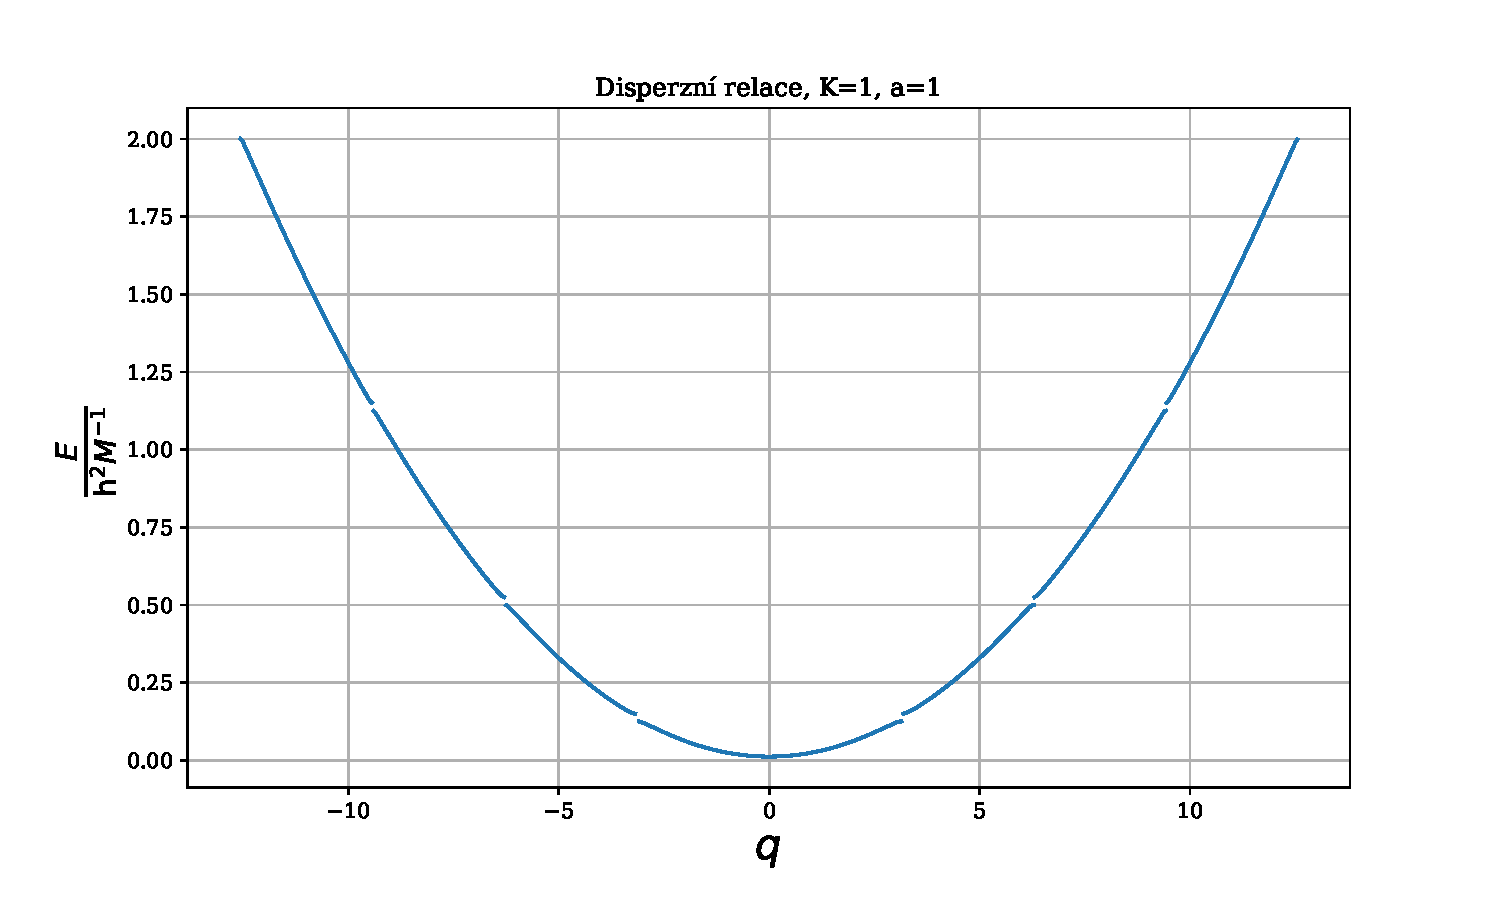
\includegraphics[scale=0.7]{disperzni1.pdf}
\end{figure}

\begin{figure}[p]
    \centering
    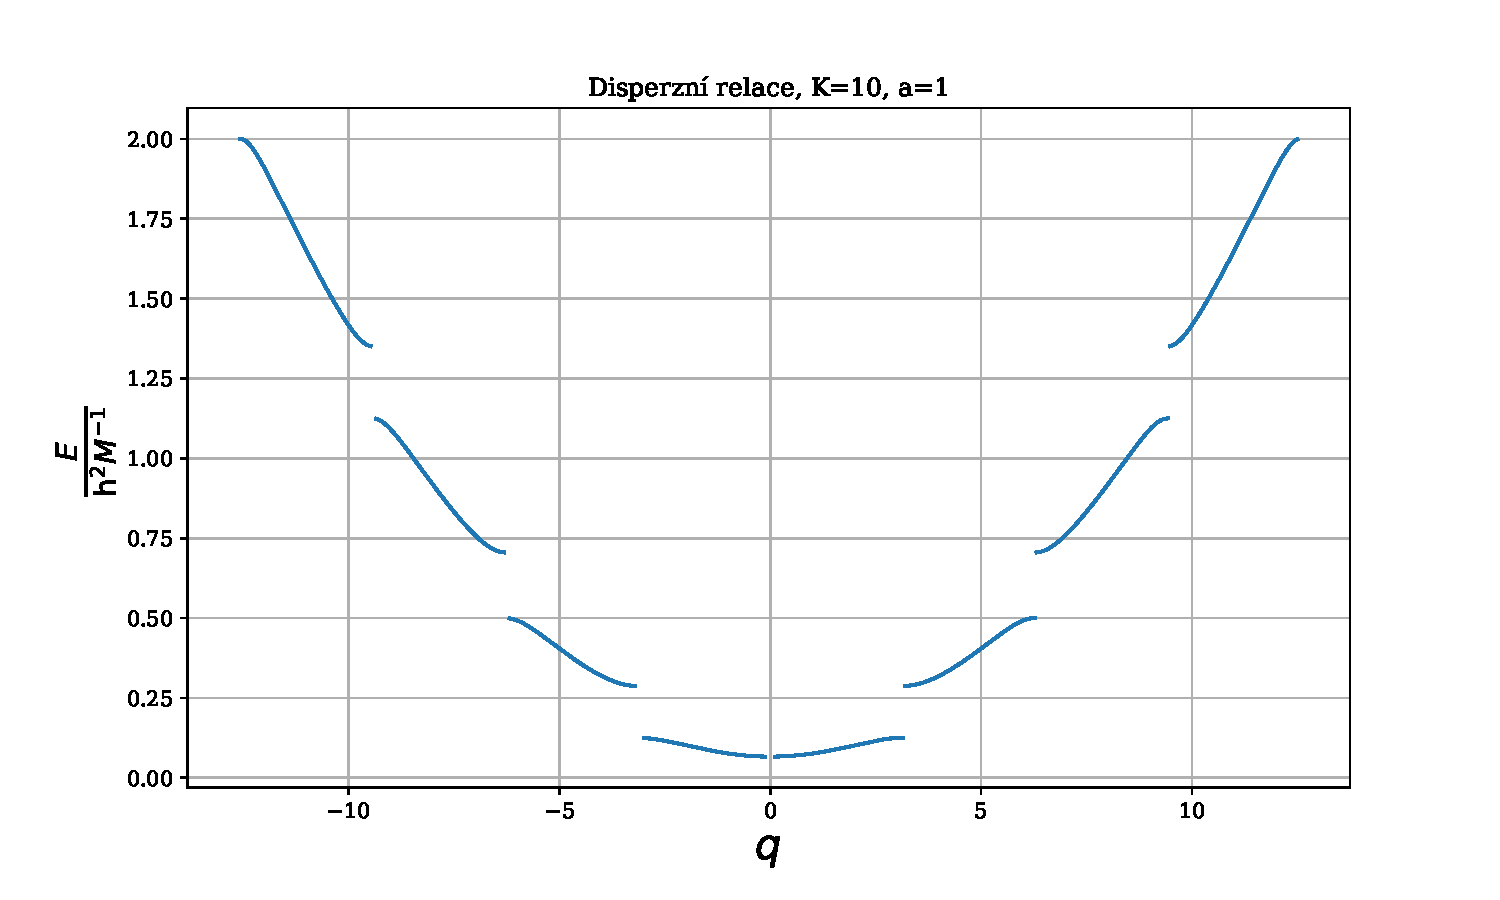
\includegraphics[scale=0.7]{disperzni10.pdf}
\end{figure}

\pagebreak

Pro vypočtení derivace využijeme implicitní funkci. Vztah $\tilde{E}(q)$ vyjádřený jako implicitní funkce má tvar:
\begin{gather*}
    \Phi_K(q, \tilde{E}) =
    \cos{qa} - \theta_K(t(\tilde{E})).
\end{gather*}
Derivace $\tilde{E}$ je potom
\begin{gather*}
    \dd{\tilde{E}}{q}(q(t)) =
    - \frac{\pd{\Phi}{q}(q(t), \tilde{E}(t))}{\pd{\Phi}{q}(q(t), \tilde{E}(t))} =
    - \frac{a \sin aq(t)}{\theta_K'(t) \; t'(\tilde{E}(t))}
    = \frac{4 \pi a^{2} t^{3} \sin{\left(a q(t) \right)}}{- 2 \pi K a t \cos{\left(2 \pi a t \right)} + K \sin{\left(2 \pi a t \right)} + 8 \pi^{2} a^{2} t^{2} \sin{\left(2 \pi a t \right)}}.
\end{gather*}
Pro grupovou rychlost $v_\const{g}$ platí:
\begin{gather*}
    v_\const{g}(q) = \frac{1}{\hbar} \dd{E}{q} = 2 \pi \frac{\const{h}}{M} \dd{\tilde{E}}{q}
\end{gather*}
Veličinu $\tilde{v}_\const{g}$ (opět podělenou konstantami) tedy můžeme v závislosti na $q$, resp. $E$ parametrizovat:
\begin{gather*}
    \phi_q(t) = \mat{
        q_K(t) \\[7pt]
        2 \pi \dd{\tilde{E}}{q}\hspace{-3pt}(q(t))
    },
    \hspace{3em}
    \phi_E(t) = \mat{
        \tilde{E}(t) \\[7pt]
        2 \pi \dd{\tilde{E}}{q}\hspace{-3pt}(q(t))
    }.
\end{gather*}
\begin{figure}[!ht]
    \centering
    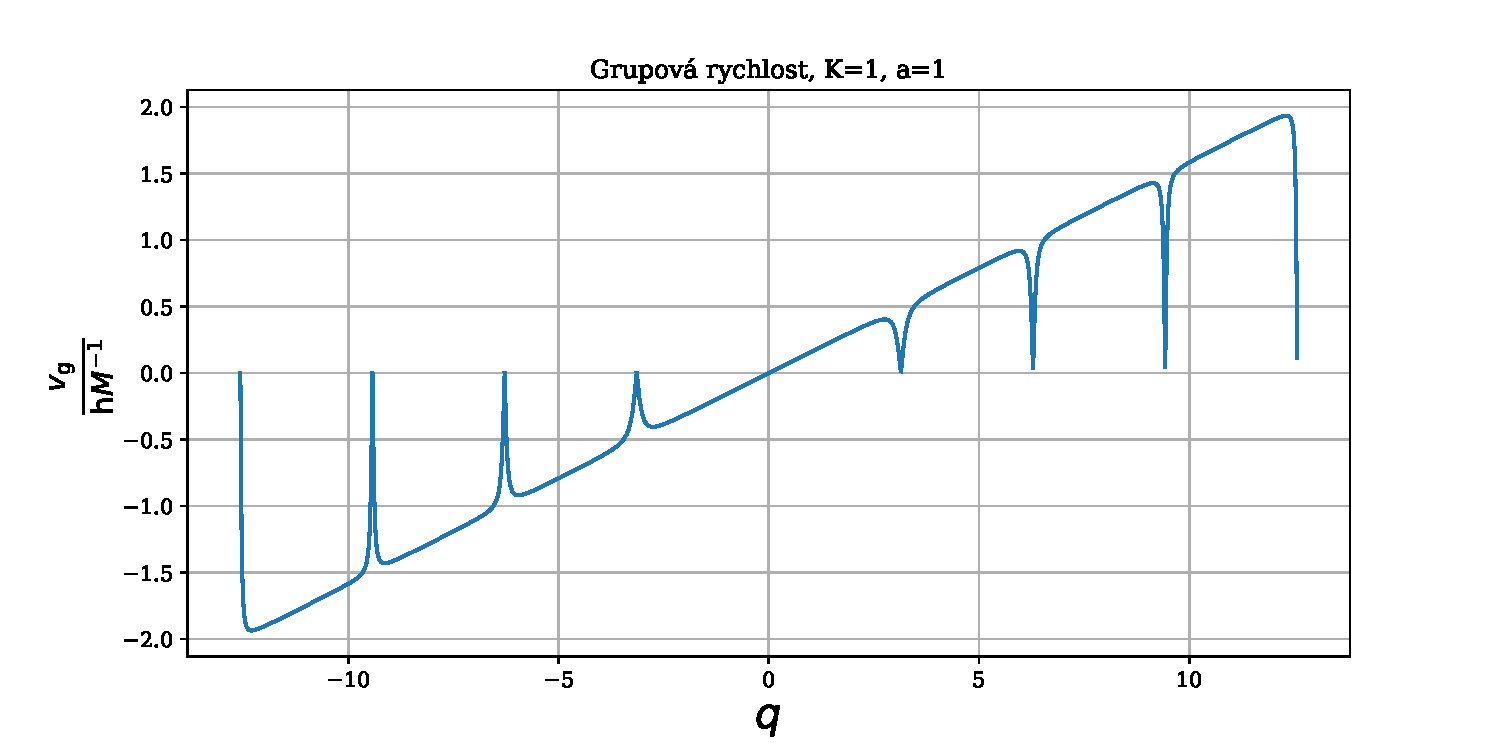
\includegraphics[scale=0.65]{grupova1_q.pdf}
\end{figure}

\begin{figure}[!ht]
    \centering
    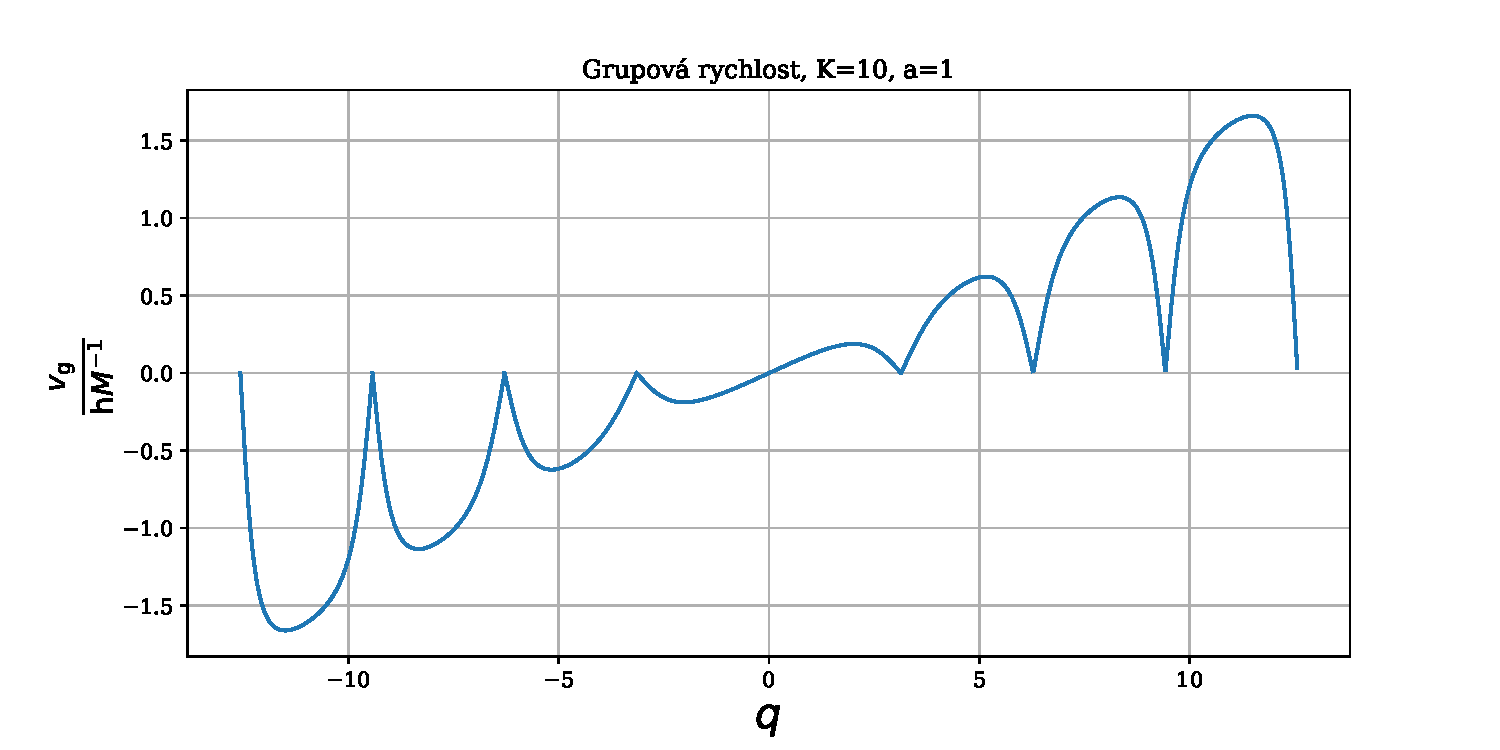
\includegraphics[scale=0.65]{grupova10_q.pdf}
\end{figure}

\begin{figure}[!ht]
    \centering
    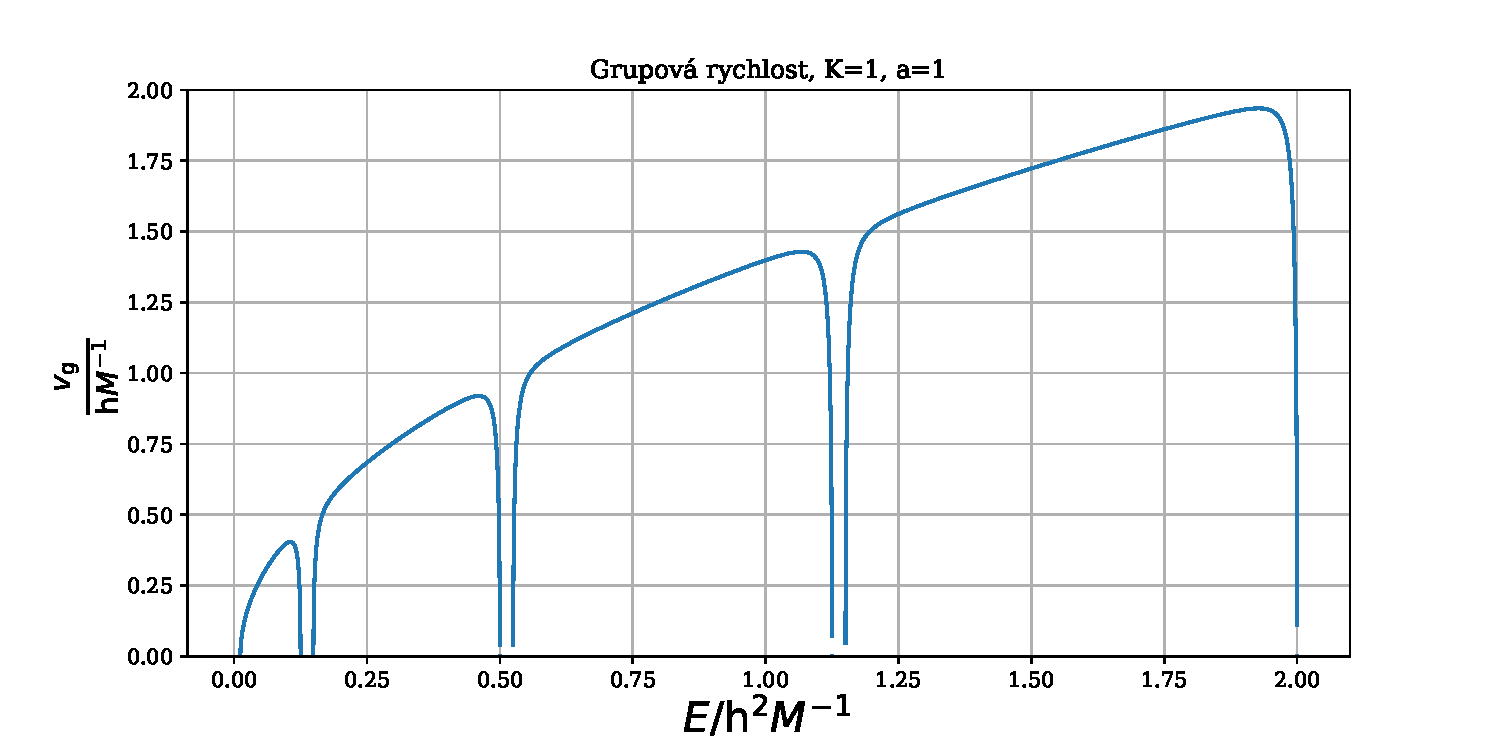
\includegraphics[scale=0.65]{grupova1_E.pdf}
\end{figure}

\begin{figure}[!ht]
    \centering
    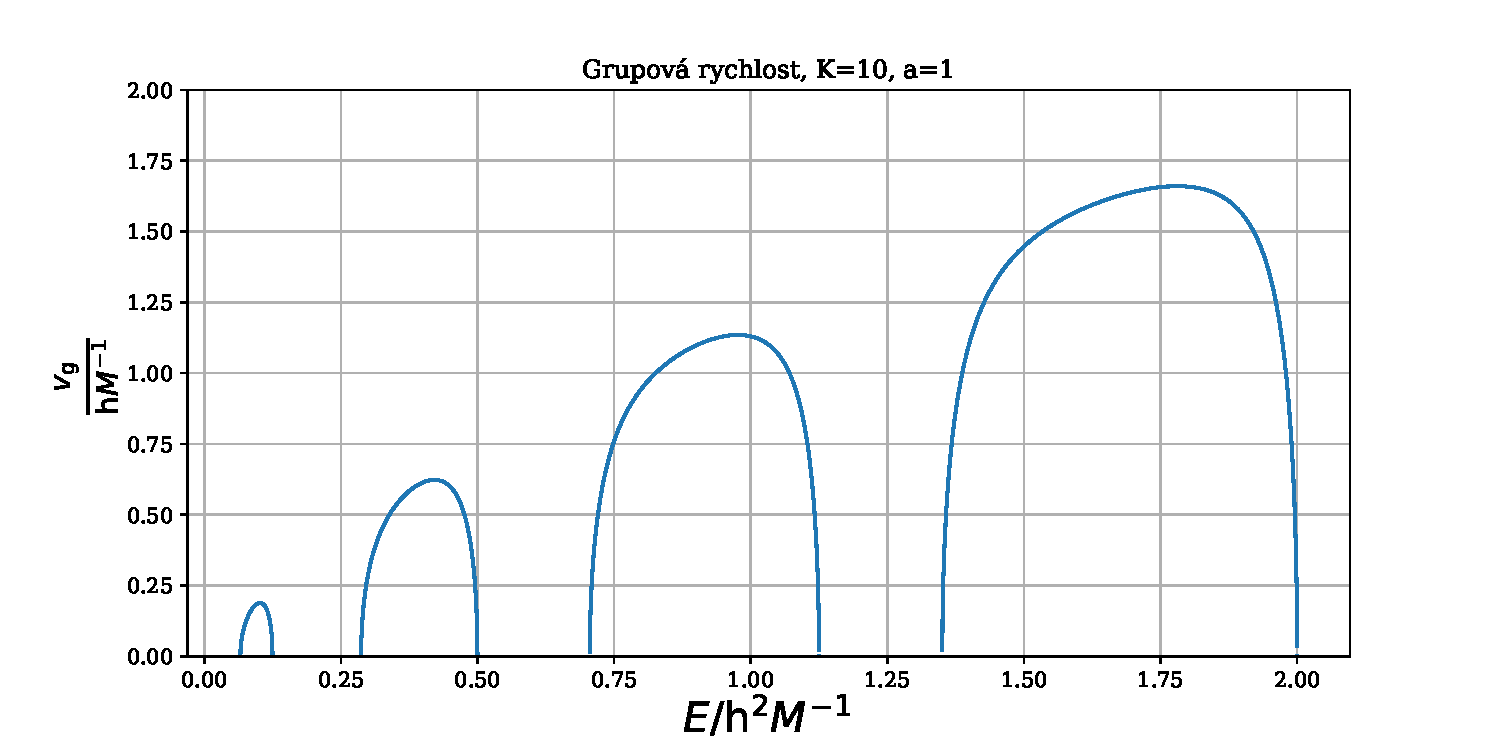
\includegraphics[scale=0.65]{grupova10_E.pdf}
\end{figure}

\subsection{Řešení pro \texorpdfstring{$E<0$}{E<0}}

Pro záporné energie máme podle Blochova teorému:
\begin{align*}
    \psi_I &= \e{\i q x} \left( A \e{-\i q x} \e{kx} + B \e{-\i q x} \e{-kx} \right), \\
    \psi_{II} &= \e{-\i q a} \left( A \e{k(x+a)} + B \e{-k(x+a)} \right).
\end{align*}
Aplikujeme-li nyní slepovací podmínky, získáme:
\begin{align*}
    \psi_{II}(0-) &= \psi{I}(0+) \\
    \e{-\i q a} \left( A \e{ka} +  B \e{-ka}\right) &= A + B
    \\[10pt]
    \psi_{II}'(0-) - \psi_I'(0+) &= - K(A+B) \\
    \e{-\i q a}\left( Ak\e{ka} - B\e{-ka} \right) -kA + kB &= -K(A+B)
\end{align*}
Získáme tedy lineární soustavu dvou rovnic, po převedení do maticové podoby:
\begin{gather}
    \mat{
        \e{-\i qa + ka} - 1 &
        \e{-\i qa - ka} - 1 \\
        k\left(\e{-\i qa + ka} - 1\right) + K &
        -k\left(\e{-\i qa - ka} - 1\right) + K
    }
    \mat{A \\ B} = 0
    \label{maticova-AB}
\end{gather}
Podmínka nulovosti determinantu vede na rovnici
\begin{gather*}
    \cos qa = \cosh ak + \frac{K}{2k} \sinh ak
\end{gather*}
Parametrizace bude zjevně téměř stejná, jako pro případ $E>0$, jenom pomocnou funkci $\theta_K(t)$ si předefinujeme:
\begin{gather*}
    \theta_K(t) = \cosh(2\pi t) + \frac{K}{2k} \sinh(2\pi t).
\end{gather*}
Nakonec ještě normalizujeme vlnovou funkci:
\begin{align*}
    \int_0^a |\psi(x)|^2 \d{x} &=
    \int_0^a \left( A\e{2kx} + 2AB + B\e{-2kx} \right) \d{x} =
    \left[ \frac{A}{2k} \e{2kx} + 2ABx - \frac{B}{2k} \e{-2kx}\right]_0^a
    \\
    &= \frac{A}{2k} \left( \e{2ka} - 1 \right) + 2aAB + \frac{B}{2k} \left( 1 - \e{-2ka} \right)
    = 1
\end{align*}
Tato rovnice společně s \eqref{maticova-AB} stačí k určení koeficientů $A, B$ pro konkrétní hodnoty $q, K, a$.

\begin{figure}[!ht]
    \centering
    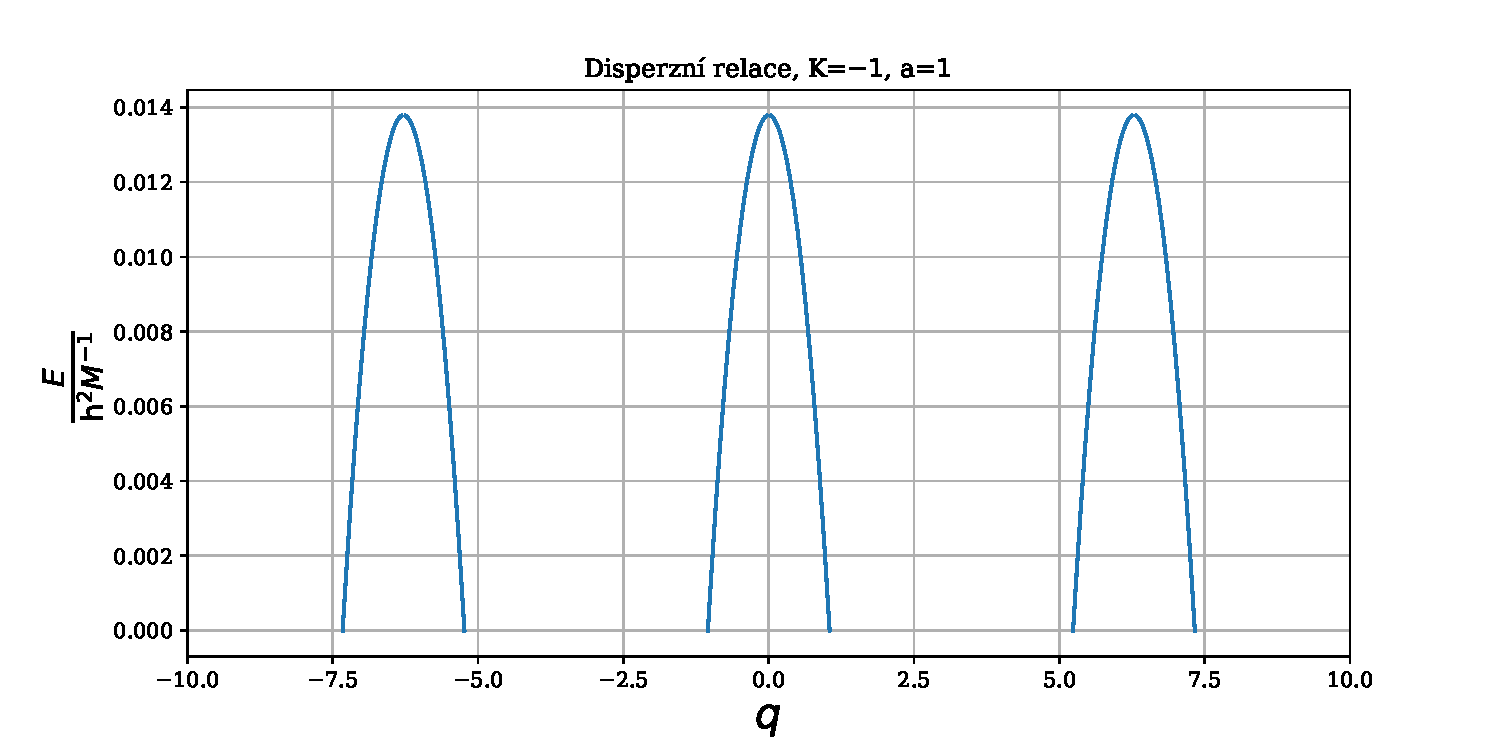
\includegraphics[scale=0.65]{disperzni-1_neg.pdf}
\end{figure}

\begin{figure}[!ht]
    \centering
    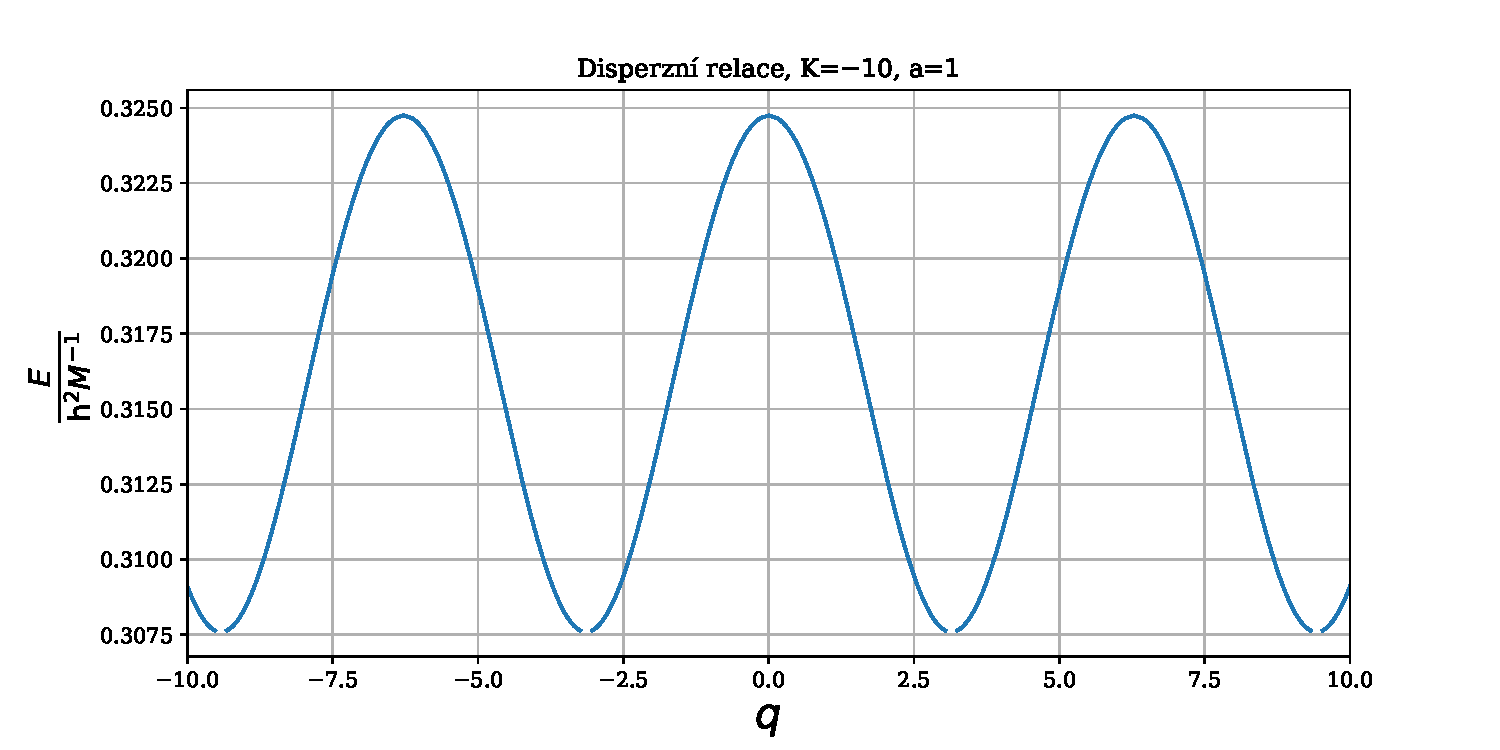
\includegraphics[scale=0.65]{disperzni-10_neg.pdf}
\end{figure}

\pagebreak

\section{Cvičení 11. 12.}
\subsection{Zadání}

Vyjádřete normalizovanou vlnovou funkci $\psi_z(x) = \braket{x}{z}$ koherentního stavu harmonického oscilátoru. Dosaďte do
\begin{align*}
    z = \sqrt{\frac{m\omega}{2\hbar}} \left( \left< \hat{x}_z \right> + \frac{\i}{m\omega} \left< \hat{p}_z \right> \right)
\end{align*}
a ukažte, že hustota pravděpodobnosti $| \psi_z(x, t) |^2$ odpovídá gaussovskému vlnovému balíku, jehož střední hodnota kmitá kolem počátku s frekvencí $\omega$, vypočtěte jeho disperzi a ukažte, že se v čase nemění. Vyjádřete normalizovanou vlnovou funkci $\tilde{\psi}_z(p) = \braket{p}{z}$.

\subsection{Řešení}
Víme, že pro koherentní stav harmonického oscilátoru platí
\begin{align*}
    \hat{a} \ket{z} = z \ket{z},
\end{align*}
vyjádříme-li si nyní operátor $\hat{a}$ jako
\begin{align*}
    \hat{a} = \frac{1}{\sqrt{2m\omega\hbar}}\left( m \omega \hat{x} + \i \hat{p} \right),
\end{align*}
dostaneme pro $\psi_z$ diferenciální rovnici
\begin{align*}
    \bra{x} \hat{a} \ket{z} &= z \braket{x}{z}
    \\
    \frac{1}{\sqrt{2m\omega\hbar}}\left( m \omega \hat{x} + \i \hat{p} \right) \psi_z &= z \psi_z
    \\
    m \omega \, x \psi_z + \hbar \psi'_z &= \sqrt{2m\omega\hbar} z \, \psi_z
    \\[5pt]
    \hbar \psi'_z &= \left( \oldsqrt{2m\omega\hbar} \, z - m \omega \, x\right) \psi_z
\end{align*}
Rovnice má triviální nefyzikální řešení $\psi_z = 0$. Zkusíme ji řešit pomocí násady $\e{a(x+b)^2}$:
\begin{align*}
    \hbar \left(2a(x+b)\right) \e{a\left(x+b\right)^2} &= \left( \oldsqrt{2m\omega\hbar} \, z - m \omega \, x\right) \e{a\left(x+b\right)^2}
    \\[3pt]
    2\hbar \, a \, x + 2\hbar \, ab &= \oldsqrt{2m\omega\hbar} \, z - m \omega \, x
\end{align*}
\begin{align*}
    2\hbar \, a \, x &= -m \omega \, x
    & 2\hbar \, ab &= \sqrt{2m\omega\hbar} \, z
    \\[5pt]
    a &= - \frac{m\omega}{2\hbar}
    & b &= \frac{\sqrt{2m\omega\hbar}}{2\hbar a} \, z
    \\[5pt]
    & & b &= - \frac{\sqrt{2m\omega\hbar}}{2\hbar} \frac{2\hbar}{m\omega} \, z
    \\[5pt]
    & & b &= - \sqrt{\frac{2\hbar}{m\omega}} \, z
\end{align*}
\begin{align*}
    \psi_z(x) \propto \exp ( \; { -\frac{m\omega}{2\hbar} \left( x - z \sqrt{\frac{2\hbar}{m\omega}} \right)^2 } \, ).
\end{align*}
Snadno můžeme rozmyslet, že diferenciální rovnici funkce $\psi_z$ splňuje, i když ji škálujeme libovolným komplexním číslem. Protože fáze vlnové funkce nemá fyzikální význam, ponecháme ji beze změny. Hledáme tedy pouze reálnou kladnou normalizační konstantu.
\begin{align*}
    1 &= \braket{z}{z} = \int_{-\infty}^{+\infty} \psi_z^* \psi_z \d{x}
    \\
    &= N^2 \int_{-\infty}^{+\infty} \exp ( \; { -\frac{m\omega}{2\hbar} \left( x - z \sqrt{\frac{2\hbar}{m\omega}} \right)^2 } \, ) \d{x}
    \\[3pt]
    &= N^2 \int_{-\infty - z \sqrt{2\oldhbar / m\omega}}^{+\infty - z \sqrt{2\oldhbar / m\omega}} \exp ( \; { -\frac{m\omega}{2\hbar} x^2 } \, ) \d{x}
    = N^2 \int_{-\infty}^{+\infty} \exp ( \; { -\frac{m\omega}{2\hbar} x^2 } \, ) \d{x}
    \\[3pt]
    &= N^2 \sqrt{\frac{2\pi\hbar}{m\omega}}
    \implies
    N = \left( \frac{2\pi\hbar}{m\omega} \right)^{\!\nicefrac{1}{4}}
\end{align*}
Normalizovaná vlnová funkce je tedy (po dosazení za $z$):
\begin{align*}
    \psi_z(x) = \left( \frac{2\pi\hbar}{m\omega} \right)^{\!\nicefrac{1}{4}} \; \exp ( \; { -\frac{m\omega}{2\hbar} \left( x - \left< \hat{x}_z \right> + \frac{\i}{m\omega} \left< \hat{p}_z \right> \right)^2 } \, ).
\end{align*}

\vspace{3em}

Nyní spočítáme hustotu pravděpodobnosti nalezení částice v poloze $x$:
\begin{align*}
    | \psi_z(x) |^2
    &= \left( \frac{2\pi\hbar}{m\omega} \right)^{\!\nicefrac{1}{2}} \; \exp ( \; { -\frac{m\omega}{2\hbar} \left( \left( x - \left< \hat{x}_z \right> \right)^2 - \left( \frac{1}{m\omega} \left< \hat{p}_z \right>\right)^2 \; \right) } \, )
    \\
    &= \left( \frac{2\pi\hbar}{m\omega} \right)^{\!\nicefrac{1}{2}} \; \exp ( \; {
        \underbrace{-\frac{m\omega}{2\hbar}}_a \; x^2 +
        \underbrace{\frac{m\omega}{\hbar} \left< \hat{x}_z \right>}_b \; x + \underbrace{\frac{1}{2m\omega\hbar} \left< \hat{p}_z \right> - \frac{m\omega}{2\hbar} \left< \hat{x}_z \right>}_c
    } \, ).
\end{align*}
Vidíme, že se jedná o gaussovskou funkci, střední hodnotu a disperzi vypočteme následovně:
\begin{gather*}
    \mu = \frac{-b}{2a} = \left< \hat{x}_z \right>,
    \hspace{4em}
    \sigma = \sqrt{ -\frac{1}{2a} } = \sqrt{\frac{\hbar}{m\omega}}.
\end{gather*}

\vspace{3em}

Pokračujeme určením časového vývoje vlnové funkce. Platí:
\begin{align*}
    \ket{z(t)} &= \hat{U}(t) \; \ket{z}
    \\
    &= \e{-\i\hat{H}\,t/\oldhbar} \; \ket{z}
    \\
    &= \e{\displaystyle -\i\omega(\hat{a}^\dagger \hat{a} + \nicefrac{1}{2}) \, t} \;\;\; \e{\displaystyle \nicefrac{|z|^2}{2}} \;\;\; \sum_{n=0}^\infty \frac{z^n}{\oldsqrt{n!}} \ket{n}
    \\
    &= \e{\displaystyle \nicefrac{|z|^2}{2}} \;\;\; \sum_{n=0}^\infty \; \frac{z^n}{\oldsqrt{n!}} \;\, \e{\displaystyle -\i\omega(\hat{a}^\dagger \hat{a} + \nicefrac{1}{2}) \, t} \; \ket{n}
    \\[2pt]
    &= \e{\displaystyle \nicefrac{|z|^2}{2}} \;\;\; \sum_{n=0}^\infty \; \frac{z^n}{\oldsqrt{n!}} \;\, \e{\displaystyle -\i\omega(n + \nicefrac{1}{2}) \, t}  \; \ket{n}
    \\
    &= \e{\displaystyle \nicefrac{|z|^2}{2}} \;\;\; \e{\displaystyle \nicefrac{-\i\omega t}{2}} \;\;\; \sum_{n=0}^\infty \frac{(z \, \e{-\i\omega t})^n}{\oldsqrt{n!}} \;\; \ket{n}
    \\
    &= \e{\displaystyle \nicefrac{-\i\omega t}{2}} \; \ket{z\e{-\i\omega t}}
\end{align*}
Dosazením do vlnové funkce dostáváme:
\begin{align*}
    \psi_z(x, t) = \left( \frac{2\pi\hbar}{m\omega} \right)^{\!\nicefrac{1}{4}} \; \exp ( \; { -\frac{m\omega}{2\hbar} \left( x - \left< \hat{x}_z \right> \, \e{-\i\omega t} + \frac{\i}{m\omega} \left< \hat{p}_z \right> \, \e{-\i\omega t} \right)^2 } \, ).
\end{align*}
Můžeme vypočíst pravděpodobnostní hustotu:
\begin{align*}
    |\psi_z(x)|^2 &= \left( \frac{2\pi\hbar}{m\omega} \right)^{\!\nicefrac{1}{2}} \; \exp ( \; { -\frac{m\omega}{2\hbar} \left( x - \left< \hat{x}_z \right> \, \e{-\i\omega t} + \frac{\i}{m\omega} \left< \hat{p}_z \right> \, \e{-\i\omega t} \right)^2 } \, ) \; \exp ( \; { -\frac{m\omega}{2\hbar} \left( x - \left< \hat{x}_z \right> \, \e{\i\omega t} - \frac{\i}{m\omega} \left< \hat{p}_z \right> \, \e{\i\omega t} \right)^2 } \, )
    \\[5pt]
    &= \left( \frac{2\pi\hbar}{m\omega} \right)^{\!\nicefrac{1}{2}} \; \exp ( \; -\frac{m\omega}{\hbar} \left(
        \left( x - \left< \hat{x}_z \right> \cos \omega t + \frac{\left< \hat{p}_z \right>}{m\omega} \sin \omega t \right)^2
        - \left( \left< \hat{x}_z \right> \sin \omega t + \frac{\left< \hat{p}_z \right>}{m\omega} \cos \omega t \right)^2
    \right) \, ).
\end{align*}
Porovnáním s pravděpodobnostní hustotou nezávislou na čase, snadno nahlédneme, že
\begin{align*}
    \sigma = \sqrt{\frac{\hbar}{m\omega}},
    \hspace{4em}
    \mu = \left< \hat{x}_z \right> \cos \omega t - \frac{\left< \hat{p}_z \right>}{m\omega} \sin \omega t.
\end{align*}
Pro vyjádření vlnové funkce v $p$-reprezentaci provedeme obdobný postup jako na začátku – nejprve si vyjádříme diferenciální rovnici, kterou vyřešíme pro $\tilde{\psi}_z(p)$.
\begin{align*}
    \frac{1}{\oldsqrt{2m\omega\hbar}} \left( -m\omega\hbar\dd{}{p} + p \right) \tilde{\psi}_z = z \tilde{\psi}_z
    \;\; \implies \;\;
    \tilde{\psi}_z(p,t) = \left( 2\pi m\omega\hbar \right)^{-\nicefrac{1}{4}} \; \exp( \; \frac{1}{2m\omega\hbar}\left( p - \sqrt{2m\omega\hbar} \; z \e{-\i\omega t} \right)^2 \, ).
\end{align*}

\end{document}